\begin{figure}[h]
    \centering
    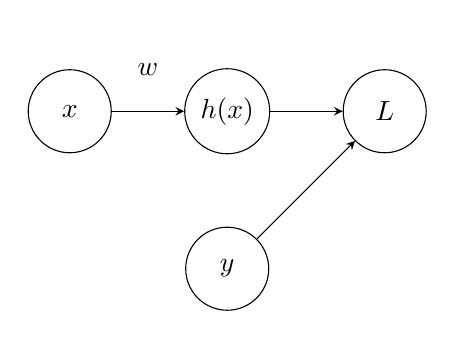
\begin{tikzpicture}[
        node/.style=draw, circle, minimum size=3em,
        forward/.style=->, >=stealth,
        scale=2
    ]
        \node[node] (x) at (0, 0) {$x$};
        \node[node] (hx) at (1, 0) {$h(x)$};
        \draw[forward] (x) edge node [midway, above] {$w$} (hx);
        \node[node] (y) at (1, -1) {$y$};
        \node[node] (l) at (2, -0) {$L$};
        \draw[forward] (hx) -- (l);
        \draw[forward] (y) -- (l);
    \end{tikzpicture}
    \caption{Linear Regression Computation Graph}
\end{figure}
